\documentclass[11pt,letterpaper]{article}
%\documentclass[11pt,a4paper]{report}

\usepackage{amssymb,amsmath,amsthm} 
\usepackage[margin=2cm]{geometry}
\usepackage{fancyhdr}
\usepackage{enumitem}
\usepackage[compact]{titlesec}
\usepackage{graphicx,ctable,booktabs,subfigure}

\usepackage{xparse,hyperref,parskip}

%\newcommand{\abs}[1]{\left|#1\right|}

\newcommand{\semester}{Spring 2022}
\newcommand{\due}{Thursday, February 3}


\pagestyle{fancy}
\lhead{ }
\chead{\footnotesize Math 3338\quad  Numerical Methods\quad  \semester}
\rhead{\footnotesize \thepage}
\setlength{\parindent}{0cm}
\setlist{noitemsep}



\input{defs.tex}

%Defines the problem environment with arguments Points and Solution gap
\input{problem_env.tex}



\begin{document}

\begin{center}
{\huge{\bf  Numerical Methods}} \\[1.5ex]
{\bf Math 3338 -- \semester}\\[1.5ex]
{\Large{\bf Worksheet 6\ \\[2ex] Integration}}\\
\end{center}
\vspace{2mm}

\section{Reading}

\begin{table}[!ht]
 \centering
 \begin{tabular}{ll}
   CP & 5.1, 5.6 \\
 NMEP & 6.2
 \end{tabular}
\caption{Sections Covered}
\end{table}



\section{Integration}

Evaluate the following,
\[
 \int_0^8(x+1)\sqrt{1-\frac{1}{2}\sin^2(x)}\,dx
\]
Remember, an integral is an area under a curve. Let's plot this graph and see how it looks. 
\begin{figure}[!ht]
 \centering
 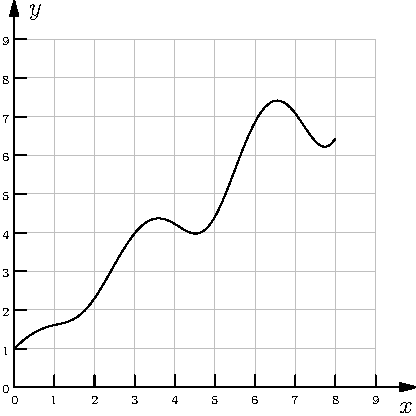
\includegraphics{images/fun.pdf}
 \caption{The graph of $(x+1)\sqrt{1-\frac12\sin^2(x)}$}
 \label{fig:fun}
\end{figure}
Figure \ref{fig:fun} does not make this function look easier to integrate.

We can't find the antiderivative of this function, I'm sorry if you tried. Luckily, we're in a 
class called Numerical Methods, so we'll evaluate this numerically. The basic idea is to approximate
the trouble function by a nicer function, and integrate that instead.

\subsection{Constant Function}
Break the interval into regions, and approximate the function by a constant in each region. Figure
\ref{fig:const} shows an example of this.
\begin{figure}[!ht]
 \centering
 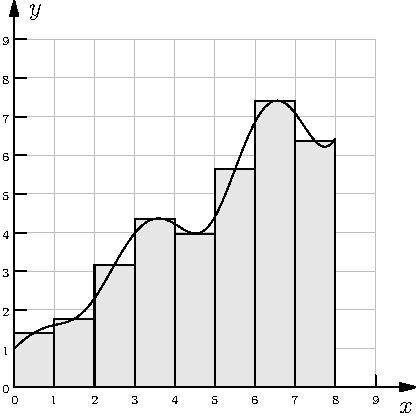
\includegraphics{images/fun_constant.pdf}
 \caption{Constant Approximation}
 \label{fig:const}
\end{figure}
you \emph{should} recognize this. 


It's a Riemann sum using midpoints. This is a nice example, the subintervals are the same width
and we're using a consistent point in each region. Mathematically, neither of these are necessary,
you can have different sized subintervals and choose whatever point your heart desires.

As a summation, this is
\[
\sum_{i=0}^{n-1} f(x_i)\Delta x
\]
where there are $n$ subintervals, $x_i$ is a point in the $i^{th}$ subinterval, and $\Delta x$ is
the width of the subintervals (assuming a constant width). Notice, $f(x_i)\Delta x$ is just
the area of a rectangle.

\subsection{Linear}
We want more accuracy! Instead of a constant function, let's approximate the function by a line.
Figure \ref{fig:trap} shows this.
\begin{figure}[!ht]
 \centering
 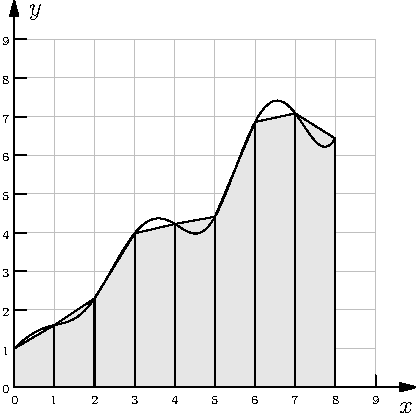
\includegraphics{images/fun_trap.pdf}
 \caption{Linear Approximation}
 \label{fig:trap}
\end{figure}

This is the trapezoid method. The area of a trapezoid is 
$\frac{(\text{height}_1+\text{height}_2)}{2}\cdot \text{base}$ (this actually makes perfect sense
if you think about it). Therefore, if there are $n$ subintervals of $[a,b]$, the trapezoid method
is,
\[
\sum_{i=0}^{n-1}\left(\frac{f(a+i\Delta x)+f(a+(i+1)\Delta x)}{2}\right)\Delta x = 
\frac12 f(a)\Delta x + \sum_{i=1}^{n-1} f(a+i\Delta x)\Delta x + \frac12 f(b)\Delta x
\]

\subsection{Quadratic}
This is Simpson's method. Figure \ref{fig:simp} shows a representation.
\begin{figure}[!ht]
 \centering
 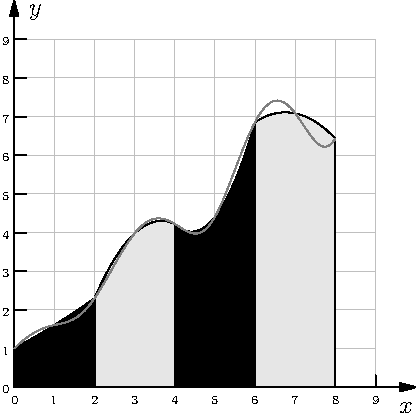
\includegraphics{images/fun_simp.pdf}
 \caption{Simpson's Method}
 \label{fig:simp}
\end{figure}
The idea is to represent the function using quadratics. However, you need 3 points to fit a 
quadratic, that's why the figure has only 4 distinct regions. This also implies you need an 
even number of subintervals, which isn't always feasible with real data. The formula is,
\[
\frac{\Delta x}{3}\left(f(x_0)+4f(x_1)+2f(x_2)+4f(x_3)+2f(x_4)+\cdots+4f(x_{2n-1})+f(x_{2n})\right)
\]
where $x_i = a+i\Delta x$.


\subsection{Higher Order}
You could proceed to approximate the function with higher order polynomials. This works, but 
is not the best way to do it. There is a method called \emph{Gaussian quadrature}. This is a 
clever method that varies the width of each interval to more accurately approximate the integral.
This is covered in detail in Section 5.6 in the text. I highly recommend reading through this.
In general, we'll black box Gaussian quadrature (we'll use it, but won't know exactly how it works).




\newpage

\begin{center}
{\huge{\bf  Numerical Methods}} \\[1.5ex]
{\bf Math 3338 -- \semester}\\[1.5ex]
{\Large{\bf Homework 6 (Due: \due)}}\\
\end{center}
\vspace{2mm}



\begin{problem}
Write three functions, \texttt{riemann}, \texttt{trapezoidal}, and \texttt{simpsons}. The functions
will have 4 inputs, a function $f$, $a$, $b$, and $N$. Your programs should be robust enough to 
handle the situations $a=b$ and $b<a$. Each of these functions should use vectorization and numpy. 

There is a Pickle file on Canvas. It's a list \texttt{[function,a,b,N,riemann,trap,simp]}. There is also a file called ``my\_functions.py''. You'll need to import this into the namespace with the pickle file \texttt{from my\_functions import *}.
\end{problem}


\begin{problem}
Let $f(x) = \int_0^x (t+1)\sqrt{1-\frac{1}{2}\sin^2(t)}\,dt$. Make a graph of $f(x)$ for 
$-5\le x\le 5$.
\end{problem}



\begin{problem}
The goal of this problem is to explore the speed of numpy vs non-numpy. Write a new trapezoidal
function \texttt{trapezoidal\_new} that doesn't use numpy (the opposite of your
original). Evaluate $\int_{-2}^2 e^{-x^2}\,dx$ using both functions and many small and large 
values of $N$, timing each trial. Make a table comparing the computation times. Discuss the results.

Note: My numpy trapezoid rule computes the integral in 0.045578 seconds for $N=1,000,000$. Yours 
should be close to this (or faster).
\end{problem}

\begin{problem}
The goal of this problem is to explore the speed of our generic \texttt{trapezoidal} method. 
Evaluate $\int_{-2}^2 e^{-x^2}\,dx$ two ways, first using our \texttt{trapezoidal} function and
second using an ad-hoc function, on where the function is within the definition of the trapezoid method. Evaluate this integral for many values of $N$, timing each trial. Make a table comparing the computation times. Discuss
the results.
\end{problem}





\end{document}




































